\documentclass[fleqn, article, a4paper]{memoir}

\usepackage[swedish]{../latex/selthcsexercise}

\usepackage[utf8]{inputenc}
% Utilities.
\usepackage{graphicx}
\usepackage{hyperref}
\usepackage{soul}
\usepackage{varioref}
\usepackage{nameref}
\usepackage{microtype}


\newcommand{\scode}[1]{\texttt{\small#1}}
\newcommand{\FIXBEFORECODE}{\vspace{-0.5\baselineskip}}
\newcommand{\FIXAFTERCODE}{\vspace{-\baselineskip}}

%---------------------------------------------------------------
\newenvironment{Hemarbete}%
{\begin{Assignments}[H]}{\end{Assignments}}

\newenvironment{Kontrollfragor}%
{\begin{Assignments}[K]\tightlist}{\end{Assignments}}

\newenvironment{Datorarbete}%
{\begin{Assignments}[D]}{\end{Assignments}}

\newenvironment{DatorarbeteCont}%
{\begin{Assignments}[D]\setcounter{Ucount}{\theSavecount}}{\end{Assignments}}

\newenvironment{Deluppgifter}%
{\begin{enumerate}[a)]\firmlist}{\end{enumerate}}

\newcommand{\commandchar}[1]{\textsc{#1}}

% Section styles.
\setsecheadstyle{\huge\sffamily\bfseries\raggedright} 
\setsubsecheadstyle{\Large\sffamily\bfseries\raggedright} 
\setsubsubsecheadstyle{\normalsize\sffamily\bfseries\raggedright} 

\setsecnumformat{} % numrera inte laborationerna
\renewcommand{\thesection}{\arabic{section}} % för referenser till laborationerna
\renewcommand{\thefigure}{\arabic{figure}}

%*****************************************************************
\begin{document}
\courseinfo{Web Programming}{\the\year}
\maketitle
\thispagestyle{titlepage}
\vspace{-4cm}

\section*{Laboratory Exercise, HTML and CSS}
\n This lab is a preparatory tutorial. It will explain some things that are assumed you know during the labs but is not covered by your previous courses. It is not mandatory and you do not need to show it to the teacher assistant but you are more than welcome to ask questions or discuss it with the teacher assistant. \emph{Learning outcomes}:
\begin{enumerate}\firmlist 
\item Understand basic web concepts.
\item Be able to write a basic HTML code, including forms.
\item Be able to write basic CSS to style a web page.
\item Get familiar with using the development tools in a web browser.
\item Understand how JavaScript can be used to manipulate the DOM.
\end{enumerate}

%\clearpage
\subsection*{The Basics}
In this tutorial you will create a smal web page containing a form. To display the web page you need a browser. The instructions assume you are using google Chrome, but any browser should work. Normally the browser fetches the HTML-code from a server on the internet, but in this tutorial we will use a file on the local computer. Copy the HTML code bellow to text file on your local computer. You can use any name, for example \emph{lab0.html}. You will create more files later, so it is good to create a directory to store all files.
\lstinputlisting[language=html]{include/start.html}
This is a minimal web page, with a title in the \code{<head>} and a single headline in the \code{<body>}. To learn more about HTML elements you can look at the video tutorials from W3C schools, \url{https://www.w3schools.com}. W3C is the organisation owning the HTML and CSS standards, so it is a reliable source for information. I recommend the HTML video tutorials for a quick overview. Mozilla also have good documentation \url{https://developer.mozilla.org/en-US/docs/Web/HTML}.

Open your HTML file in Chrome (file/open file...) and you should see a page containing a headline. If you look at the url field in the browser, it indicates that the page is loaded from a file and if you click on the url, it starts with \code{file://}. Normally the url will start with \code{https://}, secure http which is the protocol commonly used between a web server and a web browser when content is fetched from the internet.

This is a static web page. It could contain interactive forms, animations and JavaScript and still be a static page. The distinction between static and dynamic web pages is when it is generated. A static page is stored as it is viewed while a dynamic page is generated when requested, either on the server or in the web browser.

\subsection*{HTTP validation}
The page you loaded follows the HTML standard. What happens if you have an error in your code? Lets try. Change ``\code{<h1>My own form</h1>}'' to ``\code{<heading>My own form</rubrik>}'' and reload the page. There are no errors or warnings despite the error in the HTML code. The \code{<heading>} is an unknown tag name, but that is allowed. It is ignored when rendering the page. The error is \code{</rubrik>}. This is an end tag, but there is no matching start tag. The take home message here is that the browser will not warn if you have an error in the HTML code. If your page does not look as you expect, check for missing start/end tags, misspelled tag names or incorrect nesting of tags. You can also use a validator to check the HTML code, for example \url{https://validator.w3.org/}.

\subsection*{Developer tools}
How did the browser parse your incorrect HTML code? You can use the browsers developer tools to answer this question. The browser does not only show HTML pages, it is also the runtime environment for web apps. To support developers it provides good tools for monitoring and debugging web apps. In addition to the built in tools, Chrome also has a range of plugins for this, making it a popular choice among developers. This is the main reason I recommend Chrome in this course. Open the developer tools from the menu: view/developer/"Developer tools" and look at the \emph{Elements} tab. It shows the DOM, the browsers internal data structure to store the HTML code. Here you see that a \code{<heading>} element was crated with a matching end tag. The erroneous \code{</rubrik>} was discarded and is not present in the DOM. Moving the mouse pointer over the elements in the Elements tab will highlight the elements on the web page, making it easy to see which part of the page an element belongs to. You can both view and modify the DOM. Find the \code{<heading>} element, double click on "My own form" and change the text. The page is updated when you press enter. 

Another useful tab in the developers view is \emph{Network}. It shows the loading of files. Now there is only one file loaded. Edit your HTML file, add an image inside the \code{<body>} and reload it:
\begin{Code}
<img src="https://www.w3schools.com/favicon.ico" alt="w3schools logo">
\end{Code}
The logo should appear on the page, and you will see two downloads in the \emph{Network} tab. Change the url to something that does not exist, for example:
\begin{Code}
<img src="missing-url" alt="w3schools logo">
\end{Code}
Notice that the loading of ``missing-url'' is now red to indicating an error when loading. The \emph{Network} tab is the place to check that all parts of your page is loaded properly.

\subsection*{Forms}
Forms are a common mechanism for getting user input in a web app. Forms are bult using standard HTML tags. In the later labs you will learn how to read the user input in your JavaScript program but first you need to get familiar with the right HTML tags.

\medskip
\noindent \emph{Assignment 1:} Create a form for ordering a hamburger. You should be able to:
\begin{itemize}
\item choose size, one of: 90 gram, 120 gram, 180 gram
\item select add-ons, any combination of: onion, tomato, cucumber
\item place the order using a submit button
\end{itemize}
Use an validator to verify that your HTML code is correct. You can see how my form looks like in figure \ref{fig:form}.

\begin{figure}[h]
\caption{My simple hamburger form}
\label{fig:form}
\centering
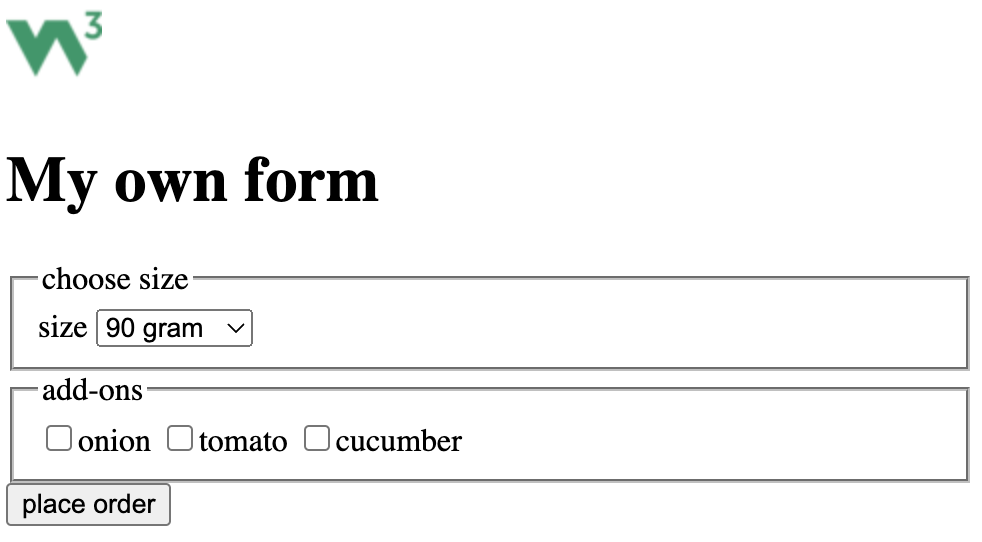
\includegraphics[height=4cm]{include/form.png}
\end{figure}

\emph{Hint:} I use the following tags \code{<form>, <fieldset>, <legend>, <label>, <select>, <option>, <input>}. You can use \code{<input>} for several types of input, check the \code{type} attribute. Check the documentation at Mozillas or W3school if you are not familiar with the tags.

What happens when you click the ``place order'' button? If you selected any of the add-ons you see that the form is cleared. Look at the \emph{Network} tab in the developer tools.  You can note that the load times varies slightly when you click on the submit button. The page is reloaded, so the form is displayed as it is defined in your HTML code rather than being reset. This is the default behaviour of a form. The browser takes all data in the form and send it to the server that the page was loaded from. The server runs a program that processes the data and generate a response, a new HTML page containing the order confirmation in this case. The browser will displays the response generated on the server. In our case the page was loaded from a file, so the browser simply discards the form data and loads the file again. Later in the course you will learn how to intervene this sequence of actions, but handling events is beyond the scope of this tutorial.

\subsection*{Accessibility and user experience}
Accessibility (A11y) means enabling as many people as possible to use websites, including those with limited abilities. The most common way to achieve this is by ensuring that assistive technologies work properly to access the content. These technologies include screen readers, screen magnifiers, speech recognition tools, and alternative input devices. How well does your page support assistive technologies? If you used the tags in the hint, then you are done. These tags have a semantic meaning and the browser will provide all information needed by the assistive tools. This is not the case when using generic tags, such as \code{<div>}. Then you need to provide additional markup for the same user experience. You do this by setting the \emph{Accessible Rich Internet Applications (ARIA)} attributes. They define the elements \emph{role} (e.g. navigation), \emph{properties} (e.g. required) and \emph{state} (e.g. the value of an input field). The \code{aria-*} attributes are beyond the scope of this tutorial.

Did you note the \code{alt} attribute in the \code{<img>} element used earlier? It provides an alternative text to the image which can be used by screen readers. It also improves the UX for users on a slow connection, they see the text while the image is loading. The alternative text is also used by search engines. You should always provide an alternative text to images, videos et.c.

A web page is commonly used as a click interface, with a mouse or trackpad as the input device. Support for other input devices is important for accessibility and user experience. It should be possible to use the web page only using a keyboard. The native form elements support this. Try it on your form, use tab to jump the input focus to the next input field, arrow key to select different options in a \code{<select>} element, space to toggle a checkbox and enter to submit the form. You need to add this functionality, as well as setting \code{aria-*} attributes, if you use other HTML tags as input fields. Forcing the user to switch between keyboard for writing text, and a mouse for clicking on buttons, is a poor user experience and poor work environment. An earlier version of LADOK was reported as work environment risk due to poor support for keyboard input. Form could not be submitted using the enter key and action buttons could not be targeted using the tab key.

The tab key do not only focus on form inputs, it iterates trough all interactive elements on a page, including for example hyper links \code{<a href="target">}. You can make any element focusable by setting the \code{tabindex} attribute. A value of 0 means both the user and your app can focus on the element. Use the elements \code{focus()} method to do this from JavaScript. A value of -1 means that the focus can be set programmatically, but not by the user. It is possible to set the cycle order among elements with different positive values of \code{tabindex}, but it is instead recommended to have a correct order of the elements in the HTML code. Try it on your page, for example by adding a \code{tabindex} to the headline, reload and use thet tab key to cycle trough the interactive elements.
\begin{Code}
<h1 tabindex="0">My own form</h1>
\end{Code}
Remember the \code{tabindex} when building navigation menus and icon/widget based interfaces.

If you want to learn more about accessibility you can for example read \url{https://developer.mozilla.org/en-US/docs/Learn/Accessibility}.

Developers should always use the correct semantic HTML element when possible, instead of setting \code{aria-*} attributes. This is the safest and easiest path to a successful suport for accessibility and good user experience.

\subsection*{CSS}
How an element is displayed is controlled by the elements style attribute. You can set the attribute directly in the element: 
\begin{Code}
<h1 style="color: red; text-align: center">My own form</h1>
\end{Code}
This sets the \code{color} and \code{text-align} style attribute, making the text centered and red. There are many attributes, see for example \url{https://www.w3schools.com/cssref/index.php} for a list.

You can set the style attribute for each element, but this becomes tedious and error prone if you want the same style to several elements. Instead CSS is commonly used. CSS is a declarative language, you define a pattern, called a selector, and all elements matching the pattern are updated, for example:
\begin{Code}
h1 {
  text-align: center;
  color: blue;
}
\end{Code}
sets the \code{color} and \code{text-align} style properties for all \code{<h1>} elements. CSS and different selectors will be covered during the lectures, but you can also follow the tutorials at W3school or mozilla to learn more about CSS. CSS can be placed in the \code{<head>} of the HTML page, either inside a \code{<style>} element, or imported from an external file using: 
\begin{Code}
<link rel="stylesheet" href="lab0.css" />
\end{Code}
A url in the HTML code can include the path to the resource to load, the CSS file in this example. If you place the CSS file in a directory called \emph{include}, then change the attribute to \code{href="include/lab0.css"}. By default the path is relative to the html file, but you can change this using the \code{<base>} tag.

\noindent \emph{Assignment 2:} Create a file \emph{lab0.css} and use it to improve the style of your form.
\emph{Hint:} I use the following style properties in figure \ref{fig:css-form}: \code{background-color, color, text-align, border-radius, padding, margin-right, margin-top, float}.

\begin{figure}[h]
\caption{My simple hamburger form with basic styling}
\label{fig:css-form}
\centering
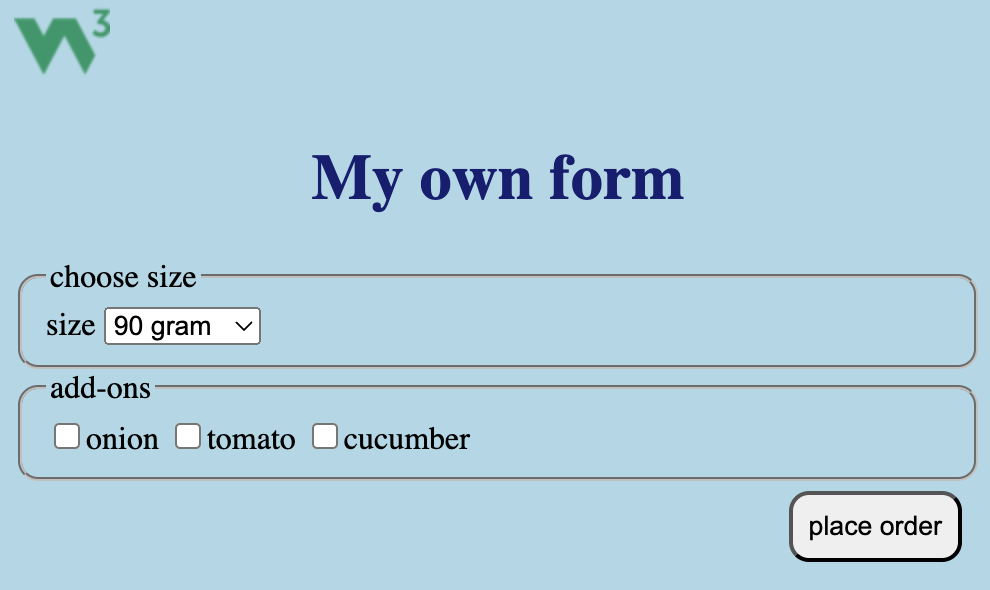
\includegraphics[height=4cm]{include/css-form.png}
\end{figure}

You do not need to write the pages design from scratch. There are several CSS templates you can use, either off the shelf or customise. Bootstrap and tailwind are popular choices. To use them you import a CSS file in a \code{<link>} and set the class attribute for all elements you want to style. This will be covered in the coming labs. Example, you can style the submit button in bootstrap using:
\begin{Code}
<input type="submit" value="place order" class="btn btn-primary">
\end{Code}

\subsection*{JavaScript}
In addition to viewing HTML pages the browser can execute JavaScript code. Inside the \code{<head>} element of your page, add:
\\\code{<script>console.log("Hello World")</script>}\\
Reload the page. Nothing changed, or? Goto the \emph{Console} tab of the developer tools. There you find the output. All printouts from your JavaScript ends up in the \emph{Console} tab. It is a good practice to always have it open when writing React apps since all warnings from React also ends up there.

You can write all your JavaScript code in \code{<script>} tags, but it quickly becomes hard to manage. Instead you commonly place the code in a separate file. Create a new file and save it as \code{lab0.js}. Add the following to it:\
\\\code{console.log("Hello from another file");}\\
Inside the \code{<head>} of your HTML file, add:
\begin{Code}
<script src="lab0.js"></script>
\end{Code}
Reload the page. You can see that it has been loaded in the \emph{Network} tab. The code is executed directly when loaded and you find the printout in the \emph{Console} tab.

JavaScript can be used to interact the DOM. You can use the global object \code{document} to access the DOM when executed in a browser. \code{document} is not declared in a non-browser environment, such as Node.js that will be used in lab 1. When present, \code{document} will always refer to an instance of the \code{Document} class. You can read and manipulate the DOM using this object. Finding elements by traversing the tree can be tedious and error prone. Instead you can search for the element using its id:
\begin{Code}
const elem = document.getElementById("my-div");
elem.innerHTML = "<h1>Hello DOM</h1>";
\end{Code}
You also need to add the element to the HTML code, anywhere inside \code{<body>} will work:
\begin{Code}
<div id="my-div">TODO</div>
\end{Code}
If you reload the page now, it will probably not work. The problem is that once \emph{lab0.js} is loaded, the script will execute, which blocks the page from rendering. This means that the rest of the content on the web page is prevented from being processed and displayed to the user until the script finishes executing. The \emph{my-div} has not been added to the DOM yet and \code{document.getElementById} will return \code{null}. Use the \code{defer} attribute to ensure that the script is executed after the page has finished loading and the DOM is built:
\begin{Code}
<script defer src="lab0.js"></script>
\end{Code}
\textbf{Warning:} the string assigned to \code{innerHTML} is parsed and added as a subtree in the DOM. The example is harmless, a \code{<h1>} element is inserted in the DOM, but this can be used to inject code to your app. Try this:
\begin{Code}
const formInput = '<img src="x" onerror="alert(\'your page has been hacked\');">';
elem.innerHTML = formInput;
\end{Code}
It is strongly advises against assigning to \code{innerHTML}. You will learn how to protect your app from code injection this later in the course.

\subsection*{Next step}
\noindent This concludes lab 0. In Lab 1 you will focus on JavaScript and in lab 2 you will develop a WebApp using React.

\input{../prechapters/licence-contributors.tex}

\end{document}
